\section{Increasing Sensitivity through PCA}\label{sec:PCA}
So far in the analysis, all features have been given an equal weighting in the beginning of training,
But, as mentioned in section \ref{sec:MLHEP}, not all features contribute to an effective signal 
region. In section \ref{subsec:PCA}, I explained how through the use of \ac{PCA}, we are able to 
create a new set of features which can be ordered by amount of variance. In this way, we can reduce
the dimensionality of the data set, while at the same time preserving most of the variance. Inn this 
section I will present the results of training on a data set which has gone through such a \ac{PCA}.
\\
In this analysis I performed a \ac{PCA} on the data set, and demanded that $99.99\%$ of the variance 
should be preserved. In doing so, 5 features were removed. Inn appendix \ref{appendix:PCA}, I have included 
the grids displaying the new sensitivity for the original signal set, using data which has gone through a \ac{PCA}. 
In figure \ref{fig:PCAComp2}, I have included two pie-plots comparing the sensitivity of the maxout (\ref{fig:MaxOutPCAComp})
and the (\ref{fig:PNNPCAComp}) with and without a \ac{PCA}.\\
\begin{figure}
    \makebox[\linewidth][c]{%
    \centering
    \begin{subfigure}{.6\textwidth}
        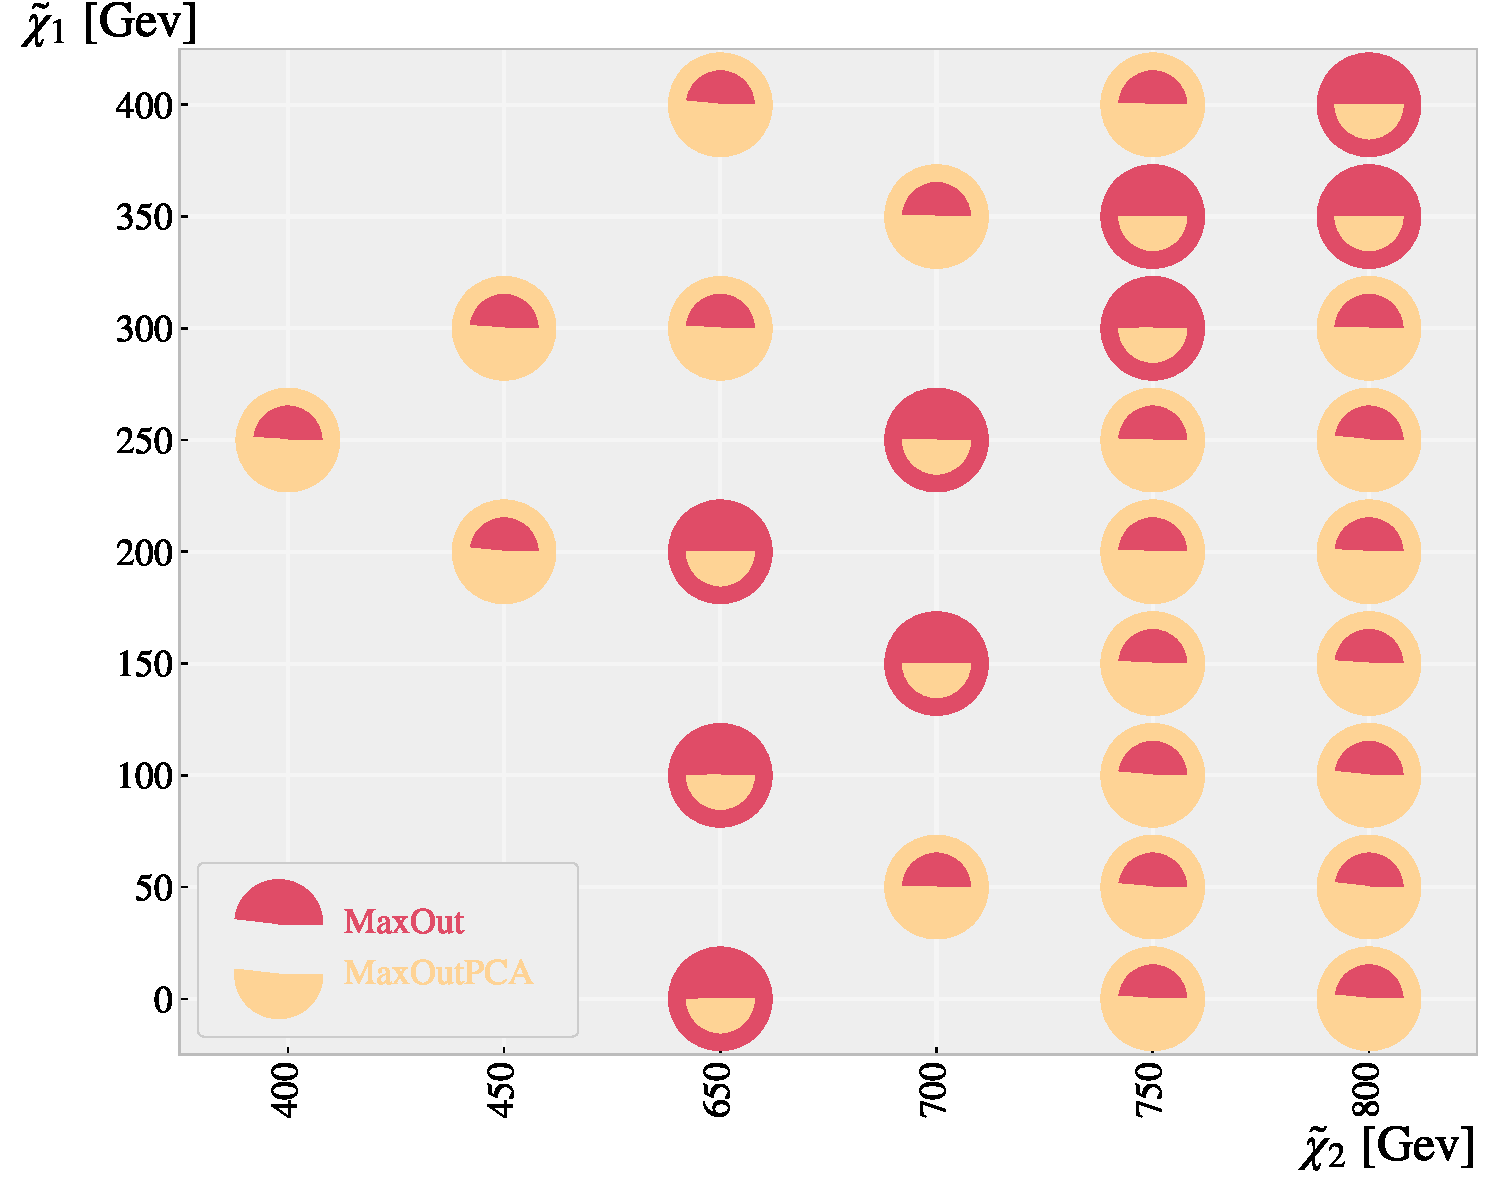
\includegraphics[width=\textwidth]{Figures/MLResults/NN/SUSY/Comparison/MaxOutPCANetworkComp.pdf}
        \vspace{-.75cm}
        \caption{}
        \label{fig:MaxOutPCAComp}
    \end{subfigure}
    \begin{subfigure}{.6\textwidth}
        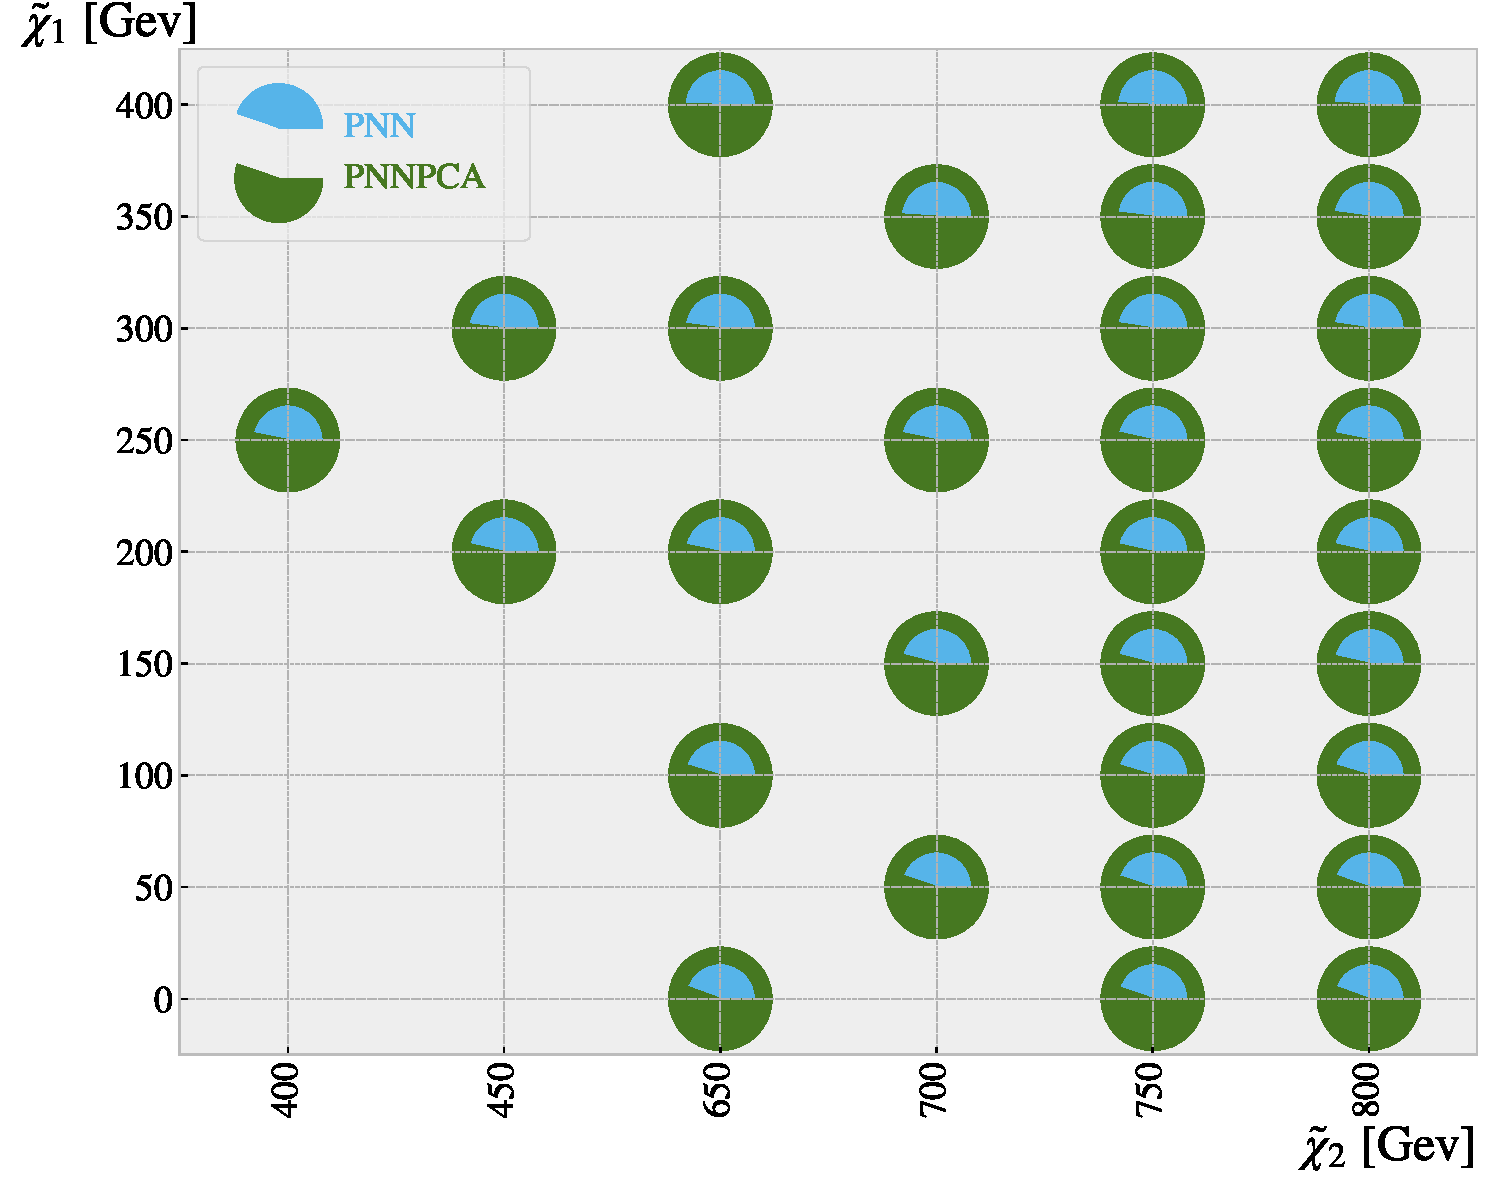
\includegraphics[width=\textwidth]{Figures/MLResults/NN/SUSY/Comparison/PNNPCANetworkComp.pdf}
        \vspace{-.75cm}
        \caption{}
        \label{fig:PNNPCAComp}
    \end{subfigure}
    }
    \caption[Two pie-plots comparing the sensitivity on the original signal set, where each figure shows the comparison between a model (maxout and \ac{PNN}) training on data 
    with and without a \ac{PCA}.]{Two pie-plots comparing sensitivity on the original signal set, where each figure shows the comparison between a model training on data 
    with and without a \ac{PCA}. Figure \ref{fig:MaxOutPCAComp} displays the comparison for the maxout model, and likewise figure \ref{fig:PNNPCAComp} 
    for the \ac{PNN}. The size of the "pie" represents the relative size of the significance and the color around each 
    point displays the method with the largest sensitivity for the respective combination.}
    \label{fig:PCAComp2}
\end{figure}
In figure \ref{fig:MaxOutPCAComp}, we can observe a relatively similar behavior with and without the \ac{PCA}. There seems to be no obvious trends in regard 
to improvement or decrease in performance for any of the mass combinations. But, to simplify the comparison between the two, we can treat all mass combinations
equally. With this in mind, maxout achieves a higher sensitivity \emph{with} a \ac{PCA} in 21/30 combinations, indicating that \ac{PCA} indeed increased performance.
Similarly, the \ac{PCA} increased performance for the \ac{PNN}, but contrary to maxout it did so for every combination in the original signal set. Additionally,
through closer study of the ratio's for each "pie", the \ac{PCA} not only increased a larger number of combinations for the \ac{PNN}, but also increased the performance
by a larger degree. Through a similar analysis, I deemed the \ac{PCA} to decrease performance for the \ac{NN}, only improving 11/30\footnote{The pie-plot comparing the 
dense \ac{NN} with and without a \ac{PCA} is included in the appendix \ref{appendix:PCA}.}. 
\\
To compare all three models discussed above with the \ac{PCA} included, I created a pie-plot which is displayed in figure \ref{fig:PCAComp}. By comparing 
the pie-plots made with and without \ac{PCA} (see figure \ref{fig:GenPlussXGB}), we notice that maxout now outperforms the dense \ac{NN} in combinations 
previously preferred by the dense \ac{NN}. Similarly, the \ac{PNN} now outperforms the maxout in three new combinations. By chance, all three of said combinations 
were combinations where the maxout model preferred no \ac{PCA}. This is yet another indication that building models to be sensitive to a large range of signals can 
sometime lead to changes which improve performance for some data, and are destructive for others. Like I mentioned in the paragraph above, I decided 
to treat all combinations equally, but with the previous point in mind, weighting the importance of certain combinations based on scientific promise/interest
could be a better approach. 
\begin{figure}
    \makebox[\linewidth][c]{%
    \centering
    \begin{subfigure}{.65\textwidth}
        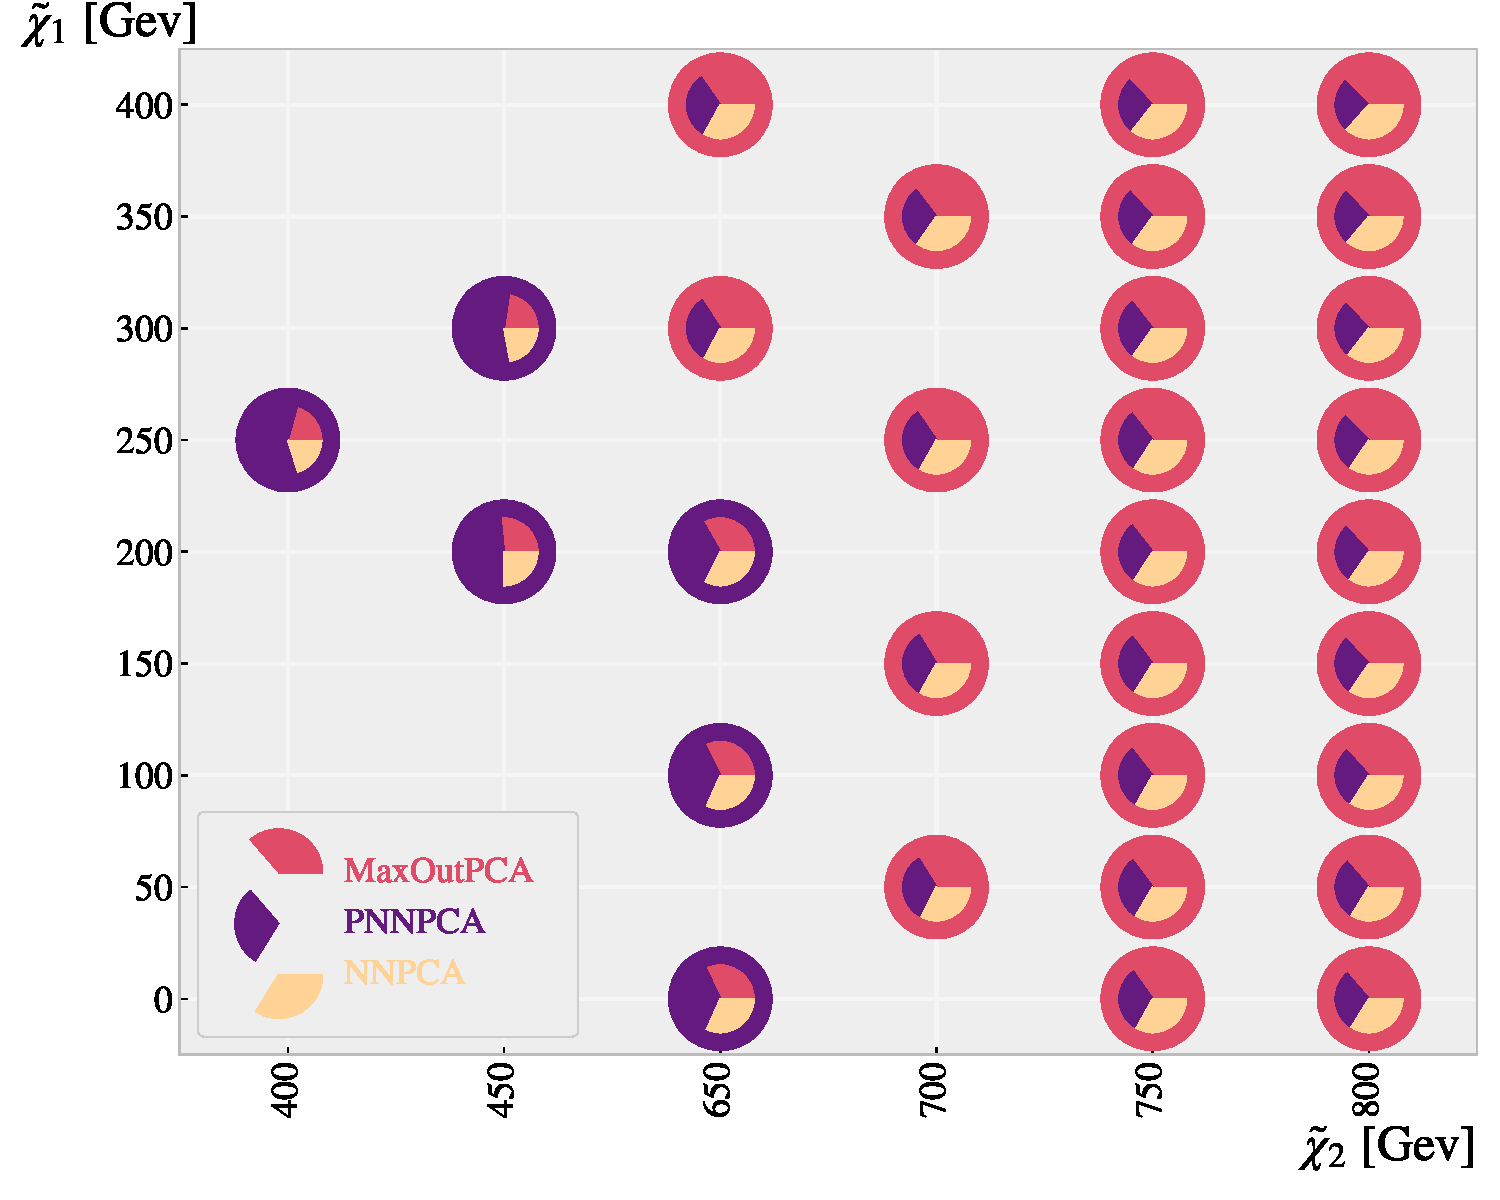
\includegraphics[width=\textwidth]{Figures/MLResults/NN/SUSY/Comparison/PCANetworkComp.pdf}
    \end{subfigure}
    }
    \caption[A sensitivity comparison between a dense \ac{NN}, \ac{PNN} and maxout  on the original 
    signal data. A \ac{PCA} analysis has been applied to the data being utilized in this result.]{A sensitivity 
    comparison between a dense \ac{NN}, \ac{PNN} and maxout on the original 
    signal data. A \ac{PCA} analysis has been applied to the data being utilized in this result. The size of the 
    "pie" represents the relative size of the significance and the color around each point displays the method with 
    the largest sensitivity for the respective combination.}
    \label{fig:PCAComp}
\end{figure}
